\documentclass[10pt]{iopart}
\usepackage{graphicx}
\usepackage{booktabs}
\usepackage{dblfloatfix}
%\newcommand{\gguide}{{\it Preparing graphics for IOP Publishing journals}}
%Uncomment next line if AMS fonts required
\usepackage{iopams}
\begin{document}


\title[B A Urazbekov \etal ]{Investigation of the Cluster Structure of $^9$Be by Reactions with a Deuteron Beam}

\author{B~A~Urazbekov$^{1,2,3,4}$, A~S~Denikin$^{2,3}$, S~M~Lukyanov$^3$,  N~Itaco$^1$,  D~M~Janseitov$^{3,4}$, K~Mendibayev$^{3,5,6}$, V~Burjan$^7$, V~Kroha$^7$, J~Mrazek$^7$, W~H~Trzaska$^8$, M~N~Harakeh$^9$, D~Etasse$^{10}$, I~Stefan$^{11}$, D~Verney$^{11}$, T~ Issatayev$^{3,5}$, Yu~E~Penionzhkevich$^{3}$, K~A~Kuterbekov$^{5}$ and T~Zholdybayev$^{6}$}

\address{$^1$ Dipartimento di Matematica e Fisica,
Universit\`{a} degli Studi della Campania “Luigi Vanvitelli”, I-8110 Caserta, Italy}
\address{$^2$ Dubna State University, 141982 Dubna, Russia}
\address{$^3$ Joint Institute for nuclear research,  141980 Dubna, Russia}
\address{$^4$ Al-Farabi Kazakh National University, 050040 Almaty, Kazakhstan }
\address{$^5$ L~N~Gumilyov Eurasian National University, 010008 Astana, Kazakhstan }
\address{$^6$ Institute of Nuclear Physics, 050032 Almaty, Kazakhstan}
\address{$^7$ Nuclear Physics Institute CAS, 25068 \v{R}e\v{z}, Czech Republic}
\address{$^8$ Department of Physics, University of Jyv\"askyl\"a, FIN-40014 Jyv\"askyl\"a, Finland}
\address{$^9$ KVI-CART, University of Groningen, 9747 AA Groningen, The Netherlands}
\address{$^{10}$ Normandie Universit\'{e}, ENSICAEN, UNICAEN, CNRS/IN2P3, LPC Caen, 14000 Caen, France}
\address{$^{11}$ Institut de Physique Nucl\'{e}aire, Univ. Paris-Sud, Universit\'{e} Paris-Saclay, F-91406 Orsay, France}
\ead{bakytzhan.urazbekov@gmail.com}

\begin{abstract}
Angular distributions of protons, deuterons, tritons and alpha particles emitted in
the d + $^{9}$Be reaction  at E$_{lab}$=19.5 and 35.0 MeV are measured.
The elastic channel is analysed in the framework of both the Optical Model and  the Coupled Channel approach.
Two kind of optical potentials are analysed: the semi-microscopic Double Folding potential and the phenomenological Woods-Saxon potential.
The deformation parameter $\beta_2$ is obtained for the transition $\frac{5}{2}^{-} \rightarrow \frac{3}{2}^{-} $ in $^9$Be.
The (d,p) and (d,t) one nucleon exchange reactions are analysed within the Coupled Reaction Channel approach.
The spectroscopic amplitudes for the nuclear reactions are calculated. Differential cross sections for the reaction channel ${^9}$Be($d$,$\alpha$)$^7$Li are calculated within the Coupled Reaction Channel method including  all possible reaction mechanisms. Corresponding contributions to the cross sections are analysed.

\end{abstract}

%
% Uncomment for keywords
\vspace{2pc}
\noindent{\it Keywords}: cluster structure, optical model, CRC, DWBA, spectroscopic amplitudes, double folding, sequential transfer
%
% Uncomment for Submitted to journal title message
%\submitto{\JPA}
%
% Uncomment if a separate title page is required
\maketitle
%
% For two-column output uncomment the next line and choose [10pt] rather than [12pt] in the \documentclass declaration
\ioptwocol
%

\section{Introduction}
The cluster structure of nuclei arises from a correlated motion of nucleons inside a nucleus. In this regime a simple subgroup can be seen as a single particle. This kind of behaviour can give insights into numerous characteristics of the nucleus, as well as affect the processes of nuclear reactions. Investigation of the cluster structure in nuclei is still one of the priority problems of modern nuclear physics in connection with the intensive developments of experimental devices.

There is a row of stable nuclei exhibiting the cluster structure, but $^9$Be is particularly worthy of attention due to the following reasons: \begin{itemize}
\item[$-$] stable nucleus with the low binding energies of neutron S$_n$=1.665 MeV, and $\alpha$-particle S$_\alpha$=2.462 MeV \cite{separationneutron};
\item[$-$] the deformed shape reflected in the nuclear quadrupole moment, Q$=+52.9 $ mb \cite{quadrupole};
\item[$-$]  the Borromean structure of the ground state;
%\item[$-$] the significant large ratio of neutrons to protons number;
\end{itemize}
These aspects led to take $^9$Be as a subject for fundamental  as well as applied researches  studies.
% Especially the latter characteristics play important role in nuclear reactor devices as a neutron moderator or  a reflector.

Regarding nuclear technologies, $^9$Be is a good wall material in thermonuclear devices \cite{kukulin2010, seksembayev2018}.
%As a rule of thumb low Z nuclei, such as $^9$Be, to have an efficient fusion fuel burning the value of admixtured material needs to be high.
%As a rule of thumb, in order to have an efficient fusion fuel burning the maximum permissible value of the admixture of wall material can be provided by low Z nuclei. %, such as $^9$Be.
%The reason is in the fact that radiation losses are caused mainly by the electronic component of the fuel and the contribution of electrons of non fuel nuclei depends directly on their Z numbers.
For instance, for fusion device types a value of some dozens of percent of soft wall material is expected in the case of $^9$Be \cite{seksembayev2018}.
The nucleus  has been chosen as it represents the best compromise based  on its ability to be well split into two energetic $\alpha$-particles by the use of $\gamma$ and $e^-$, which are efficient promoters of thermonuclear burning. Since they can be confined by electromagnetic fields and their energy affects the temperature of the burning zone.

	Scattering of the simplest projectile, such as $^{1,2}$H or $^{3,4}$He, on a target is a standard tool for fundamental study the structure of nuclei.
	This method involves measuring the angular distribution of the nuclear reaction products.
	It is well known that the energy and angular distributions of projectile-like particles give information about internal structure of target-like nuclei.
	
	In our previous works \cite{lukyanov2014, lukyanov2015, janseitov2018} the $^3$He interaction with $^9$Be was studied and angular distributions of the reaction products in the following exit channels: $^3$He+$^9$Be, $^5$He+$^7$Be, $^5$Li+$^7$Li, $^6$Be+$^6$He, and $^6$Li+$^6$Li, were measured. The obtained data were analysed within the framework of the Optical Model (OM), the Coupled Channel (CC) and the distorted wave Born approximation (DWBA) approaches  .
	The performed analysis of the experimental data showed  sensitivity of cross section on the potential parameters in the exit channels.
	Moreover, these experiments were designed to study the breakup reactions with $^9$Be in attempt to determine contributions of the channels through the $^8$Be+n  and  $^5$He+$\alpha$ structure within the inclusive measurements.
	It was found that the ratio 2.7~$\div$~1 could be assigned to the contributions of these two channels respectively. The determined value justifies that the $^5$He+$\alpha$ breakup channel plays an important role as well.

Based on the Borromean structure of $^9$Be, special attention was focused on the breakup processes resulting in the $^9$Be($^6$Li, $^6$Li)$^9$Be$^*$ nuclear reaction \cite{brown2007, papka2007}. The excited nucleus $^9$Be$^*$ can decay either directly into the $\alpha+\alpha+n$ three-body system or through one of the unstable nuclei, such as $^5$He and $^8$Be. Thereby, these relatively recent experimental studies explicitly confirm the cluster structure of $^9$Be.
The calculated branching ratios  show that the low lying excited states, at E$_x <$~4.0 MeV,  are mostly populated with the $^8$Be+n configuration. In other case, the $^5$He+$\alpha$ configuration plays a significant  role.

Another aspect of finding the cluster structure is its attandance in the nuclear reaction mechanisms. Indeed, since the papers of Detraz \etal~\cite{detraz1970, detraz1974}, the multiparticle-multihole structures have been expected at rather low excitation energies in nuclei. In this case, it can be understood that the nucleons are transferred as a whole strongly correlated cluster, which has the internal quantum numbers of a free particle.

The interaction of deuteron and alpha particles with $^9$Be was studied with regard to the cluster structure \cite{urazbekov2016, urazbekov2017}. The interaction potential of colliding nuclei was built within the framework of the Double Folding model using the three body wave function. Approbation of the double folded potential was carried out within the OM, DWBA at laboratory energies $~$10-30 MeV/nucleon. Comparison of theoretical cross sections with experimental data led to the applicability of the double folding potential based on the three body wave function.

The current work devouted to the investigation of the cluster structure of the $^9$Be nucleus studing the nuclear reactions caused by a deuteron beam at 19 MeV and 35 MeV energies. In the exit channel the simplest particles, such as p, d, t, and $\alpha$-particles, were registered and their angular distributions were obtained.
%Regarding  the previous work \cite{urazbekov2017}, we have extended our studies by adding the $^9$Be(d,$\alpha$)$^7$Li nuclear reaction, in which  two-step processes can  occur.
A comparative analysis of experimental data and theoretical calculations has been performed.
	

\section{Experimental Method}
The experiment has been performed at  the INP (\v{R}e\v{z}, Czech Republic) and  in the Physics Department of Jyv\"{a}skyl\"{a} University (Jyv\"askyl\"a, Finland).  The beam energy of $^2$H ions produced from the cyclotrons were at energies 19.5 and 35 MeV. The average beam current during the experiment was maintained at 20 nA. The self-supporting $^9$Be target was prepared from a thin beryllium foil with the 99~\% purity. A set of four telescopes was used with the purpose of registering the simplest particle of output channels. Each telescope was  contained the $\Delta$E$_0$, $\Delta$E, E$_r$ detectors with the respective thickness of 12 $\mu$m, 100 $\mu$m and 3 mm.
%%%%%%%%%%%%%%%%%%%%%%%%%%%%%%%%%%%%%
To detect reaction product in narrow divergence,  telescopes were mounted at a distance of $\sim$25 cm from the target. Each telescope was shielded by a Cu-Pb collimator with thickness of 3 mm and hole with diameter of 3 mm. The telescopes were mounted on rotating supports, which allow us to obtain data from $\theta_{lab}$ = 20$^\circ$ to 107$^\circ$ in steps of 1-2$^\circ$.

\begin{figure}[tp]
\centering
\includegraphics[width=8.2cm]{dE_E.eps}
\caption{Particle identification plots for the products of the $^{2}$H+$^9$Be reaction: $p$, $d$, $t$, and $^{4}$He. $\Delta$E is the energy loss and E$_r$ is the residual energy. Excited states for the $^7$Li reaction channel $^7$Li+$\alpha$ are indicated.}
\label{fig1}
\end{figure}

\begin{figure}[tp]
 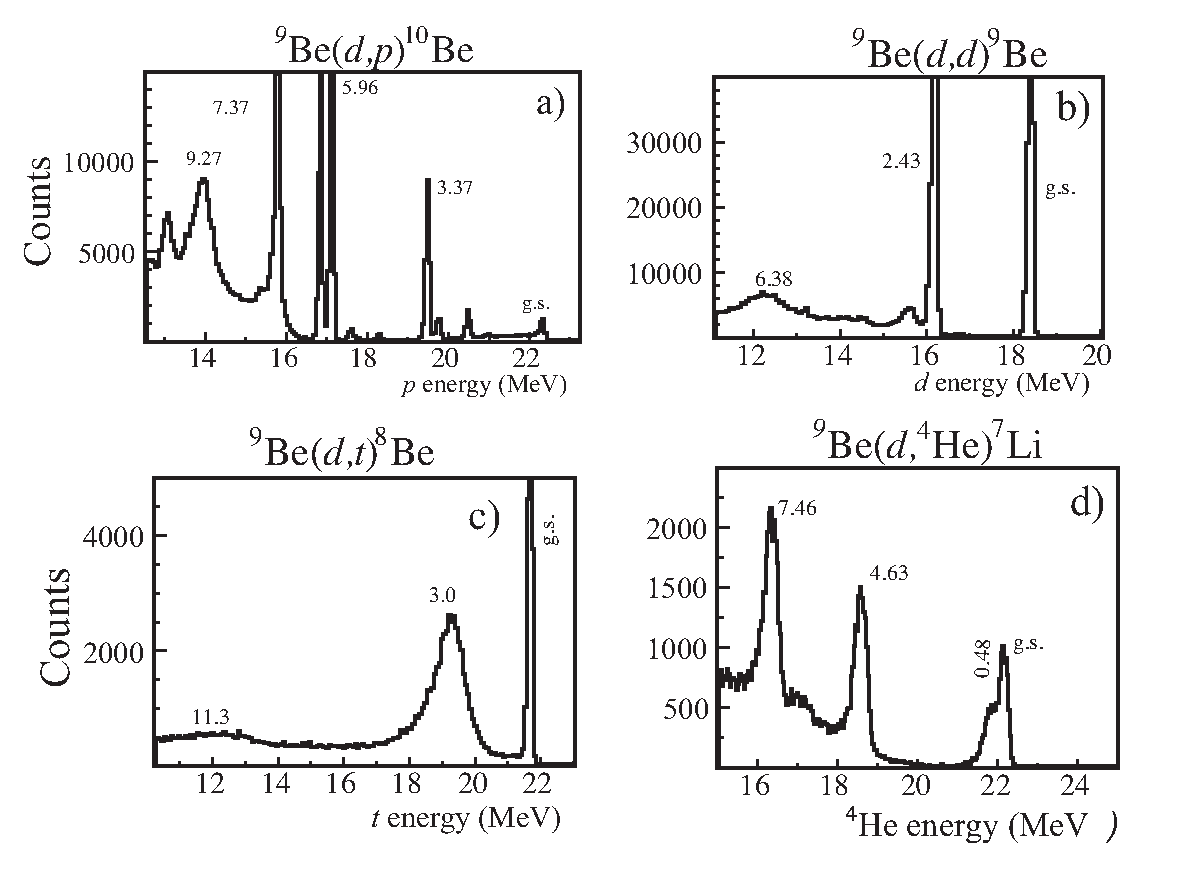
\includegraphics[width=8.2cm]{d_Etot_Fig2.eps}
\caption{Total deposited energy spectra measured at $\theta_{lab}$=32$^\circ$ for the detected $p$ (panel a), $d$ (panel b), $t$(panel c), and $\alpha$(panel d). The ground and the excited states of $^7$Li for the detected complementary product $\alpha$ as well as the ground states and the excited states for $^8$Be, $^9$Be, and $^{10}$Be in the case of detected $t, d$, and $p$, as complementary products, respectively, are unambiguously identified.}
\label{fig2}
\end{figure}	

%%%%%%%%%%%%%%%%%%%%%%%%%%%%%%%%
The particles were identified based on the energy-loss measurements of $\Delta$E and the residual energy E$_r$, i.e., by the so-called $\Delta$E-E method. An example of two-dimensional plots (yield vs. energy loss $\Delta$E and residual energy E$_r$) is shown in Fig.~\ref{fig1}.

The capability of current experimental technique is in identification of the particles $p, d, t$, and $\alpha$ and in the determination of their total deposited energies. The spectra of total deposited energy are shown in Fig.~2. All the peaks from Fig.~\ref{fig2} has been identified and assigned to the ground and the excited states of the $^{10}$Be, $^9$Be, $^8$Be, $^7$Li nuclei as the complementary products for the detected particles $p, d, t$, $\alpha$, respectively.

\section{Data Analysis and Results }
\subsection{Elastic scattering}



\begin{table*}[bp]
\footnotesize
\caption{\label{potpar}  Potential parameters of the d+$^9$Be system used in the OM, the CC and the DWBA calculations.  }
\begin{tabular*}{\textwidth}{l l  @{\extracolsep{\fill}} l l l l l l l l l l l  l}
\br
E$_d$, &The           &	$V_0$, &	$r_V^{a)}$, & $a_V$,  & $W^D_0$, &$r_D^{a)}$, &	$a_D$, & $V^{SO}_0$, & $J_V^{b)}$,           & $J_W^{b)}$		 & $\chi^2$/2 \\
MeV		& potential & MeV		&    fm	   & fm         & MeV		       & fm	    & fm	         & MeV              & MeV fm$^3$ & MeV fm$^3$		& ~	 \\
\mr
19.5 & DF	& \multicolumn{3}{c}{ $N_R=1.93^{ ~c)}$} &  14.89 &  0.630	&  0.854 & 5.56 &	617.4 &   69.7 & 	7.3	 \\
35.0 &  DF	& \multicolumn{3}{c}{ $N_R=1.81^{ ~c)}$} &   14.89	& 0.630&  0.88	& 5.56 &	587.7 & 71.2 & 	5.2	 \\
 19.5	& 	WS	& 61.97	 & 0.799	&  0.707 &  7.45	& 0.762	& 1.044 & 5.52 & 575.7 & 51.4  & 	4.8 \\
  35.0& WS	& 58.01	 & 0.799	&  0.707 &  7.52	& 0.762	& 1.044 & 5.52 & 435.1 & 51.8 & 3.4	  \\
19.5 & CC 	& 77.87	 & 0.831	&  0.780 &  7.12	& 0.816	& 0.802 & 2.8 & 690.9 & 47.2 & 	8.4  \\
35.0& CC 	& 73.9	 & 0.752	&  0.770 &  7.47	& 0.816	& 0.802 & 2.8 & 524.0 & 49.6 & 	7.1 \\
\br
\end{tabular*}
\scriptsize

$^{a)}$ The DF potential was taken as a real volume part of the optical potential with the normalization parameter $N_R$.  \\
$^{b)}$ The volume integrals are divided to the number of nucleons in colliding nuclei.
\\
$^{c)}$ Radii of the potential were defined as $R_i = r_i \left( A^{1/3}_P+A^{1/3}_T \right)$.  \\
\end{table*}

The theoretical calculations  of the deuteron  elastic scattering  on  $^9$Be  at 19.5 and 35 MeV energies have been made in the framework of the OM. The model suggests interaction between two colliding nuclei in the following way:

\begin{equation}\label{eqn:OP}
\begin{array}{l}
 U(R)=-V^{V}(R)-iW^{V}(R)+iW^D(R)+\\
~~~ ~~~~~~~+V^{SO}(R)( \mathbf{l} \cdot \sigma )+V^C(R),
\end{array}
\end{equation}
where $V^{V}, W^{V}, W^D, V^{SO},$ and $V^C$ are volume, imaginary volume and surface, spin-orbit and Coulomb potentials, respectively. In this work the real part of the optical potential were used in two forms, firstly the double folding potential (DF)
\begin{equation}
V^V(R) = N_R V^{DF}(R)
\end{equation}
with normalization factor $N_R$ and, secondly the phenomenological Woods-Saxon (WS) potential:
\begin{eqnarray}
V^V(R) =  V^V_0 f^{R_V, a_V}(R), \\
 f^{R_V,a_V}(R)=\frac{1}{1+exp{\frac{R-R_V}{a_V}}}.
\end{eqnarray}

\begin{figure}[tp]
\centering
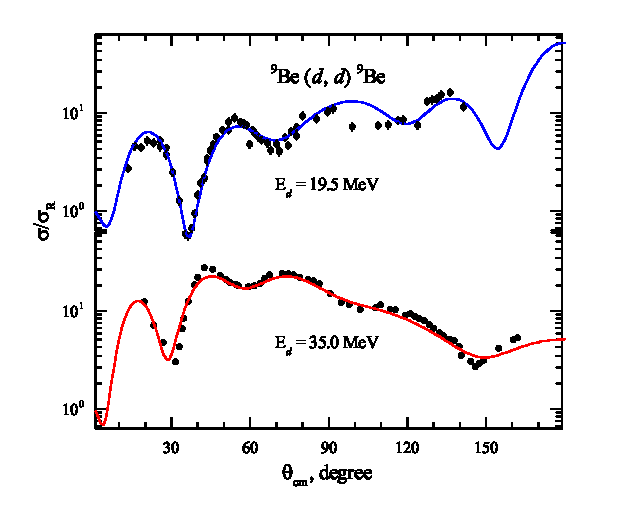
\includegraphics[width=8.2cm]{2H9BE.eps}
\caption{ \label{2H9BE}  \footnotesize The angular distributions of elastic scattering data of d from $^9$Be at laboratory energies 19.5~MeV (full circle) and 35~MeV (full triangle) in comparison with theoretical calculations within optical and couple channel model.}
\end{figure}


The DF potential was calculated using the effective M3Y-Paris nucleon-nucleon potential and the nuclear-matter-densities of projectile and target nuclei. Particularly we applied the $\alpha+\alpha+n$ three body model in order to obtain density distribution of the $^9$Be nucleus \cite{urazbekov2016}.

\begin{figure}[tp]
\centering
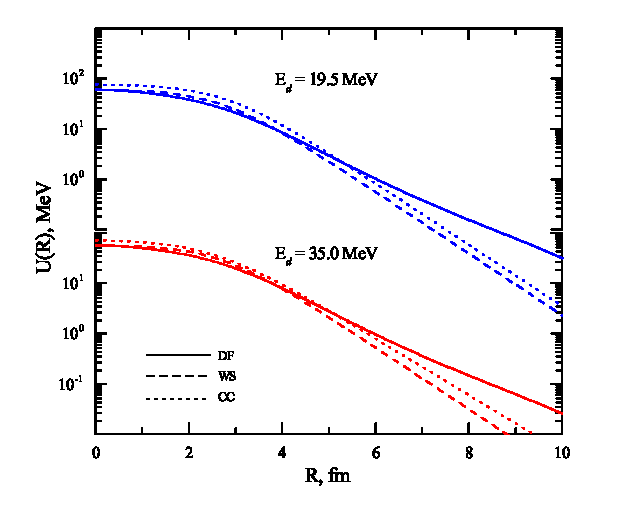
\includegraphics[width=8.2cm]{POT.eps}
\caption{ \label{POT}  \footnotesize Radial dependence of the real part of the nuclear potentials used in the elastic scattering analysis. }
\end{figure}

The surface and spin-orbit terms have standard form
\begin{eqnarray}
W^D(R) &= -4 a_D W_0^D \frac{d}{dR} f^{R_D,a_D}(R), \\
V^{SO}(R) &= V_0^{SO}\left(\frac{\hbar}{m_\pi c}\right)^2 \frac{1}{R} \frac{d}{dR} f^{R_{SO} a_{SO}}(R).
\end{eqnarray}
This form of the imaginary component of the optical potential was used for all the forms of the real one. The Coulomb term has been taken as the interaction of a point-charge with a uniformly charged sphere
\begin{eqnarray}
\label{coul}
V^C(R)=
\cases{
\frac{Z_1 Z_2 e^2}{2 R_C} \left( 3- \frac{R^2}{R_C^2} \right) & for  R $\leq R_C$ \\
 \frac{Z_1 Z_2 e^2}{R} & for  R $> R_C$\\
 }
\end{eqnarray}

The parameters of the real and imaginary parts of the optical potential were obtained fitting the theoretical cross sections to the experimental data at 19.5 MeV and 35 MeV energies. As a starting point one of the available global parametrization \cite{globalDeuteron} was used. The potential parameters obtained after fitting are listed in Table \ref{potpar}.

The measured elastic scattering cross sections are plotted in Fig.~\ref{2H9BE} in the scale of the ratio to Rutherford cross
section in comparison with the theoretical curves corresponding to the OM calculations using the DF potential (solid curve), the WS potential (dashed curve) and the CC potential (dotted curve).  Figure \ref{POT} shows the real parts of the different nuclear potentials used here.

A specific feature of the DF potential in comparison with the empirical ones is slow descending in peripheral region $r \geq 6$ fm. This is due to the broad matter density distribution of the valence neutron in $^9$Be, which also decreases slowly \cite{urazbekov2016}.

The CC potential was taken within the Coupled Channels approach that reproduces the cross section of elastic scattering and inelastic scattering data well. The coupling scheme includes the $\frac{3}{2}^-$ground and  $\frac{5}{2}^-$, $\frac{7}{2}^-$ excited states and spin re-orientations of $^9$Be.
It is interesting to note that the values of volume integrals (see Tab. \ref{potpar}) of the CC potential are different over other potentials: the real part is larger and the imaginary part is smaller. It follows from the explicit inclusion of the d+$^9$Be$^{\frac{5}{2}^-, \frac{7}{2}^-}$ inelastic channels in the analysis, which are transferred from the imaginary space to the real space. This kind of behaviour corresponds to the optical theorem.

%It also should  be noted that the potentials have almost identical behaviour in the region of the contact of colliding nuclei $\sim3.5-4.0$ fm. % Странное заключение, для 19 МэВ заметное расхождение во всей области!

The potentials obtained in this way provide quite good description of the elastic scattering cross section.


\begin{figure}[tp]
\centering
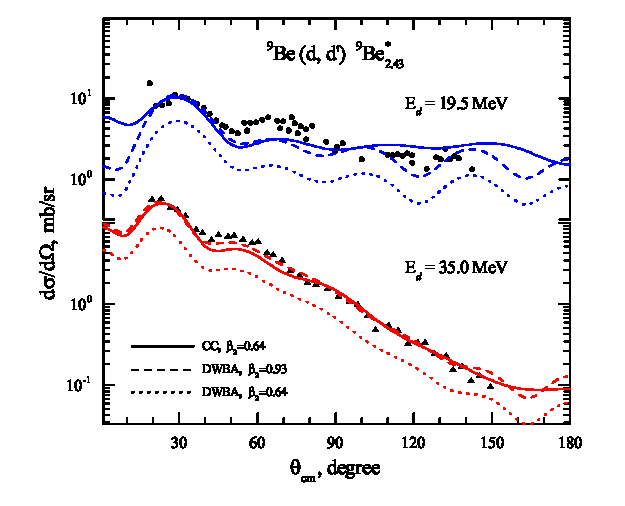
\includegraphics[width=8.2cm]{2H9BE2430MEV.eps}

\caption{\label{2H9BE2430MEV}The cross sections of inelastic scattering $^9$Be(d,d)$^9$Be* (E$_{exc}$=2.43 MeV) at laboratory energies 19.5 MeV (full circle) and 35 MeV (full triangle). Theoretical curves are described in the text.}
\end{figure}

\subsection{Inelastic scattering}
The CC and the DWBA approaches have been applied to analyse the inelastic scattering data corresponding to the excitation of the J$^{\pi}$=$\frac{5}{2}^-$ state with $E^*$ = 2.43 MeV in the ${}^9$Be target. Calculations were performed employing the $FRESCO$ code \cite{fresco} and the DWUCK5 code available on $NRV$ knowledge-base \cite{nrv}.

In order to describe obtained experimental data one consider the deformed ${}^9$Be nucleus having the quadrupole deformation and the main rotational band in the excitation spectrum including the ground state, $\frac{5}{2}^-$ state at 2.43 MeV and $\frac{7}{2}^-$ state at 6.38 MeV. All these states were included into the coupling scheme within the couple channel approach. The spin reorientations were also taken into account. The coupling interaction has the usual form:
\begin{equation}
V_\lambda(R)=-\beta_\lambda R_V \left|\frac{d V^V}{dR}\right| - i \beta_\lambda R_W \left|\frac{d W^D}{dR}\right|,
\end{equation}
where $\beta_\lambda$ is the deformation parameter of $\lambda$ multipole describing the target-nucleus form. Here we as usual neglect the contribution of the Coulomb interaction.

The calculated cross sections for inelastic scattering are shown in Fig.~\ref{2H9BE2430MEV}. The solid curves correspond to the results obtained within the CC approach, while the dashed and dotted curves were obtained within the DWBA approach using  different values of the deformation parameter $\beta_2$. The parameters of the CC potential are listed in Table~\ref{potpar}.

All the results in Fig.~\ref{2H9BE2430MEV} are in good agreement with experimental data. The quadrupole deformation parameter $\beta_2 = 0.64$ extracted within couple channel model is in consistence with the previous studies \cite{lukyanov2014, harakeh1980}.

In the case of DWBA calculations one use the DF potential (see Table~\ref{potpar}) for both the entrance and the exit channels. The DWBA angular distributions very well reproduce the structure of experimental data but distinctly underestimate them when the deformation parameter $\beta_2 = 0.64$ is used (see the dotted curves in Fig.~\ref{2H9BE2430MEV}). In order to get the best fit the deformation parameter must be increased up to $\beta_2 = 0.93$ which is quite close to the values reported in previous studies (see, for example, \cite{bodek1989, votava1973}).

\begin{figure}[bp]
\centering
\includegraphics[scale=0.85]{9BE8BECC.eps}
\caption{ \label{9BE8BECC} The target coupling schemes in the $^9$Be(d,p)$^{10}$Be (upper) and the $^9$Be(d,t)$^8$Be (lower) nuclear reactions. The bold two headed arrows indicate E$\lambda$ transitions. The spin re-orientation effects are indicated as back pointing arrows.}
\end{figure}	

Thus one may confirm that channel coupling and the effects of spin re-orientation enhance the cross section that results in the reduction of the deformation parameter. However, the DWBA approach takes into account only first order contributions to the transition amplitude. In particular, it also describes only general features of the angular distributions and overestimates the deformation parameter in order to compensate the difference between the experimental data and the DWBA cross sections.

%The implementation of the CC approach is demonstrating a good agreement with angular distributions of inelastic scattering data. Exact matching value of the deformation parameter with other theoretical researches has been obtained. Generally it can be concluded that  strong coupling effects between channels exist in $^9$Be(d,d)$^9$Be$^*$.
%In accordance with a good agreement of experimental data with both theoretical angular distributions and obtained deformation parameter within the CC approach it should therefore be noted that there exist strong coupling effects between channels.


\subsection{One nucleon transfer reactions }
The one neutron pick-up ${}^9$Be(d,t)${}^8$Be and stripping ${}^9$Be(d,p)${}^{10}$Be reactions were analyzed here within the framework of  the Coupled Reaction Channels (CRC).

\begin{figure}[tp]
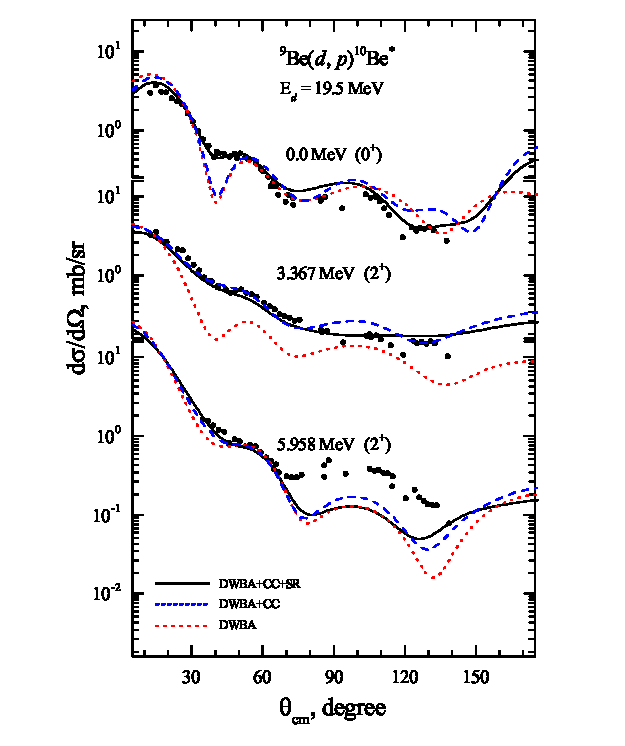
\includegraphics[scale=0.8]{1H10BE.eps}
\caption{\label{1H10BE} Differential cross sections for the ground and low-lying excited states of $^{10}$Be  produced in the d + $^9$Be nuclear reaction at 19.5 MeV. Experimental data are in comparison with  theoretical results obtained with the CRC method.  }
\end{figure}

\begin{figure}[tp]
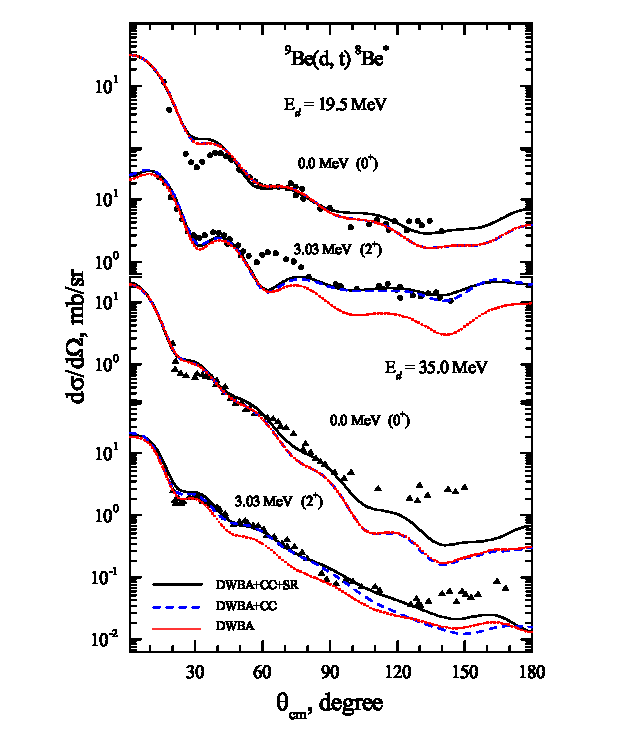
\includegraphics[scale=0.8]{3H8BE.eps}
\caption{
\label{3H8BE}
Differential cross sections of the ground and low-lying excited states of $^{8}$Be produced in the d + $^9$Be reaction at both 19 MeV and 35 MeV energies. The experimental data are shown in comparison with  theoretical results calculated within the CRC method.}
\end{figure}

The couple channel potentials given in Table \ref{potpar} were used in the CRC calculations for the entrance channel as well as the global optical parametrizations from Ref. \cite{globalProton, globalTriton} were used for the exit channels. The coupling schemes of target nuclei for the ${}^9$Be(d,p)${}^{10}$Be and ${}^9$Be(d,t)${}^8$Be  reactions  are illustrated in Fig. \ref{9BE8BECC}. The states of ${}^{10}$Be, $2^+_{1}$ and $2^+_{2}$, as well as the low-lying excited states of ${}^8$Be, $2^+$ and $4^+$, were implemented to the coupling scheme. Also, the schemes take into account the spin reorientation effects of states on the condition $J \neq 0$.

In order to construct the bound state wave functions of the transferred particle in entrance and exit channels one employed the common method, i.e. fitting the depth of the corresponding Woods-Saxon potential to the known binding energy. The reduced radius and diffuseness in this case are set to be equal $r = 1.25$ fm and $a$ = 0.65 fm correspondingly. If the transfer takes place to the final unbound states, the depth of the potential for this state was adjusted to provide the binding energy equal to $-0.1$ MeV in accordance with the recommendation given in Ref. \cite{harakeh1980}.

%If the core and the composite nuclei have internal excitation energies, a renewed binding energy $BE^{\star}$ of the transferred particle is expressed by the formula:
%\begin{equation} BE^{\star}=BE - E_{com}^*+E_{core}^* \end{equation}
%where $BE$ $-$ the binding energy of the transferred particle, $E_{com}^*,~E_{core}^*~-$  excitation energies of the composite and  core nuclei, respectively.

The spectroscopic amplitude  $\mathcal{S}$ for an addition of particle from a Core $J_{core}$ to a Composite $J_{com}$ is related to the matrix element of the creation operator~$\hat{a}^\dagger$ :
%\cite{brown2017}:
\begin{eqnarray}\label{eq:SA}
\mathcal{S}_{NL_J} = \frac{\langle J_{com} \| \hat{a}^\dagger _{NL_J} \| J_{core}  \rangle}{\sqrt{2J_{com}+1}}
%= (-)^{j+J-J'} \frac{\langle J_{core}  \| \hat{a} _{NL_J} \| J_{com}  \rangle}{\sqrt{2J+1}}
\end{eqnarray}
where $NL_J$ is the set of particle quantum numbers. The spectroscopic amplitudes for one particle states were calculated by means of the $ANTOINE$ code \cite{antoine}  using the effective Cohen-Kurath interaction for $p$-shell nuclei \cite{cohen1965}. The calculated spectroscopic amplitudes for the one nucleon transfer reactions are listed in Tab.~\ref{SA}.

\begin{table*}[tp]
\footnotesize
\caption{\label{SA} Spectroscopic amplitudes used in CRC calculations for the Composite = Core + Cluster system. The one nucleon spectroscopic amplitudes calculated by means of the $ANTOINE$ code \cite{antoine}. The alpha spectroscopic amplitudes were taken from  \cite{volya, volya2017}. }
\begin{tabular*}{\textwidth}{@{\extracolsep{\fill}}llllllrl@{\extracolsep{\fill}}llllllr@{\extracolsep{\fill}}}
\br
Composite & 2J$_{com}$ & Core & 2J$_{core}$ & Cluster & 2J & SA &    & Composite & 2J$_{com}$ & Core & 2J$_{core}$ & Cluster & 2J & SA      \\
\mr
$^9$Be  & 3  & $^8$Be   & 0   & n       & 3   & $-$0.761 &  & $^9$Be  & 3  & $^8$Li   & 2$_1$    & p       & 1   & $-$0.444  \\
$^9$Be  & 3  & $^8$Be   & 4   & n       & 3   & 0.816  &  & $^9$Be  & 3  & $^8$Li    & 6   & p       & 3   & $-$0.592  \\
$^9$Be  & 3  & $^8$Be   & 4   & n       & 1   & $-$0.242 &  & $^9$Be  & 3  & $^8$Li    & 2$_2$   & p       & 3   & $-$0.236  \\
$^9$Be  & 5  & $^8$Be   & 4   & n       & 3   & 0.986  &  & $^9$Be  & 3  & $^8$Li    & 2$_2$   & p       & 1   & 0.036   \\
$^9$Be  & 5  & $^8$Be   & 4   & n       & 1   & $-$0.417 &  & $^9$Be  & 5  & $^8$Li    & 4   & p       & 3   & 0.593   \\
$^9$Be  & 5  & $^8$Be   & 8   & n       & 3   & $-$0.374 &  & $^9$Be  & 5  & $^8$Li    & 4   & p       & 1   & 0.515   \\
$^9$Be  & 7  & $^8$Be   & 4   & n       & 3   & $-$0.457 &  & $^9$Be  & 5  & $^8$Li   & 2$_1$    & p       & 3   & $-$0.672  \\
$^9$Be  & 7  & $^8$Be   & 8   & n       & 3   & 0.919  &  & $^9$Be  & 5  & $^8$Li    & 6   & p       & 3   & $-$0.571  \\
$^9$Be  & 7  & $^8$Be   & 8   & n       & 1   & $-$0.429 &  & $^9$Be  & 5  & $^8$Li    & 6   & p       & 1   & $-$0.171  \\
$^8$Be  & 0  & $^7$Li   & 3   & p       & 3   & $-$1.204 &  & $^9$Be  & 5  & $^8$Li    & 2$_2$   & p       & 3   & 0.200     \\
$^8$Be  & 0  & $^7$Li   & 1   & p       & 1   & 0.736  &  & $^9$Be  & 7  & $^8$Li    & 4   & p       & 3   & $-$0.323  \\
$^8$Be  & 4  & $^7$Li   & 3   & p       & 3   & $-$0.748 &  & $^9$Be  & 7  & $^8$Li    & 6   & p       & 3   & $-$0.899  \\
$^8$Be  & 4  & $^7$Li   & 3   & p       & 1   & $-$0.612 &  & $^9$Be  & 7  & $^8$Li    & 6   & p       & 1   & $-$0.564  \\
$^8$Be  & 4  & $^7$Li   & 1   & p       & 3   & 0.667  &  & $^7$Li  & 3  & $^6$Li   & 2   & n       & 3   & 0.657   \\
$^8$Be  & 4  & $^7$Li   & 7   & p       & 3   & 0.624  &  & $^7$Li  & 3  & $^6$Li   & 2   & n       & 1   & $-$0.538  \\
$^8$Be  & 4  & $^7$Li   & 5$_2$   & p       & 3   & 0.079  &  & $^7$Li  & 3  & $^6$Li   & 6   & n       & 3   & 0.744   \\
$^8$Be  & 4  & $^7$Li   & 5$_2$   & p       & 3   & $-$0.146 &  & $^7$Li  & 3  & $^6$Li   & 4   & n       & 3   & $-$0.032  \\
$^8$Be  & 8  & $^7$Li   & 7   & p       & 3   & 0.864  &  & $^7$Li  & 3  & $^6$Li   & 4   & n       & 1   & 0.399   \\
$^8$Be  & 8  & $^7$Li   & 7   & p       & 1   & 0.687  &  & $^7$Li  & 1  & $^6$Li   & 2   & n       & 3   & $-$0.925  \\
$^8$Be  & 8  & $^7$Li   & 5$_2$   & p       & 3   & 0.374  &  & $^7$Li  & 1  & $^6$Li   & 2   & n       & 1   & 0.197   \\
$^8$Li  & 4  & $^7$Li   & 3   & n       & 3   & $-$0.988 &  & $^7$Li  & 1  & $^6$Li   & 4   & n       & 3   & $-$0.555  \\
$^8$Li  & 4  & $^7$Li   & 3   & n       & 1   & 0.237  &  & $^7$Li  & 7  & $^6$Li   & 6   & n       & 3   & $-$0.936  \\
$^8$Li  & 4  & $^7$Li   & 1   & n       & 3   & 0.430   &  & $^7$Li  & 7  & $^6$Li   & 6   & n       & 1   & 0.645   \\
$^8$Li  & 4  & $^7$Li   & 7   & n       & 3   & $-$0.496 &  & $^7$Li  & 7  & $^6$Li   & 4   & n       & 3   & $-$0.456  \\
$^8$Li  & 4  & $^7$Li   & 5   & n       & 3   & $-$0.665 &  & $^7$Li  & 5$_2$  & $^6$Li   & 2   & n       & 3   & $-$0.650   \\
$^8$Li  & 4  & $^7$Li   & 5$_2$   & n       & 1   & $-$0.275 &  & $^7$Li  & 5$_2$  & $^6$Li   & 6   & n       & 3   & 0.732   \\
$^8$Li  & 2$_1$  & $^7$Li   & 3   & n       & 3   & 0.567  &  & $^7$Li  & 5$_2$  & $^6$Li   & 6   & n       & 1   & 0.549   \\
$^8$Li  & 2$_1$  & $^7$Li   & 3   & n       & 1   & 0.351  &  & $^7$Li  & 5$_2$  & $^6$Li   & 4   & n       & 3   & 0.200     \\
$^8$Li  & 2$_1$  & $^7$Li   & 1   & n       & 3   & 0.905  &  & $^7$Li  & 5$_2$  & $^6$Li   & 4   & n       & 1   & $-$0.114  \\
$^8$Li  & 2$_1$  & $^7$Li   & 1   & n       & 1   & 0.331  &  & $^6$Li  & 2  & d     & 2   & $\alpha$     & 0   & 0.907  \\
$^8$Li  & 2$_1$  & $^7$Li   & 5$_2$   & n       & 3   & 0.767  &  & $^6$Li  & 2  & d     & 2   & $\alpha$     & 4   & 0.077   \\
$^8$Li  & 6  & $^7$Li   & 3   & n       & 3   & 0.581  &  & $^6$Li  & 6  & d     & 2   & $\alpha$     & 4   & 0.943   \\
$^8$Li  & 6  & $^7$Li   & 5$_2$   & n       & 3   & $-$0.660  &  & $^6$Li  & 6  & d     & 2   & $\alpha$     & 8   & 0.028   \\
$^8$Li  & 6  & $^7$Li   & 5$_2$   & n       & 1   & $-$0.541 &  & $^6$Li  & 4  & d     & 2   & $\alpha$     & 4   & 0.929   \\
$^8$Li  & 6  & $^7$Li   & 7   & n       & 3   & 0.973  &  & $^9$Be  & 3  & $^5$He   & 3   & $\alpha$     & 0   & $-$0.925  \\
$^8$Li  & 6  & $^7$Li   & 7   & n       & 1   & $-$0.404 &  & $^9$Be  & 3  & $^5$He   & 3   & $\alpha$     & 4   & 0.784   \\
$^8$Li  & 2$_2$  & $^7$Li   & 3   & n       & 3   & $-$0.617 &  & $^9$Be  & 5  & $^5$He   & 3   & $\alpha$     & 4   & 0.974   \\
$^8$Li  & 2$_2$  & $^7$Li   & 3   & n       & 1   & $-$0.841 &  & $^9$Be  & 5  & $^5$He   & 3   & $\alpha$     & 8   & $-$0.260   \\
$^8$Li  & 2$_2$  & $^7$Li   & 1   & n       & 3   & 0.178  &  & $^9$Be  & 7  & $^5$He   & 3   & $\alpha$     & 4   & 0.882   \\
$^8$Li  & 2$_2$  & $^7$Li   & 1   & n       & 1   & 0.331  &  & $^9$Be  & 7  & $^5$He   & 3   & $\alpha$     & 8   & $-$0.737  \\
$^8$Li  & 2$_2$  & $^7$Li   & 5   & n       & 3   & 0.231  &  & $^7$Li  & 3  & t     & 1   & $\alpha$     & 1   & 0.970       \\
$^9$Be  & 3  & $^8$Li    & 4   & p       & 3   & $-$0.947 &  & $^7$Li  & 1  & t     & 1   & $\alpha$     & 1   & 0.961       \\
$^9$Be  & 3  & $^8$Li    & 4   & p       & 1   & $-$0.319 &  & $^7$Li  & 7  & t     & 1   & $\alpha$     & 3   & 0.952       \\
$^9$Be  & 3  & $^8$Li    & 2$_1$   & p       & 3   & 0.454  &  & $^7$Li  & 5$_2$  & t     & 1   & $\alpha$     & 3   & 0.223  \\
\br
\end{tabular*}
\end{table*}

\begin{figure*}[bp]
\centering
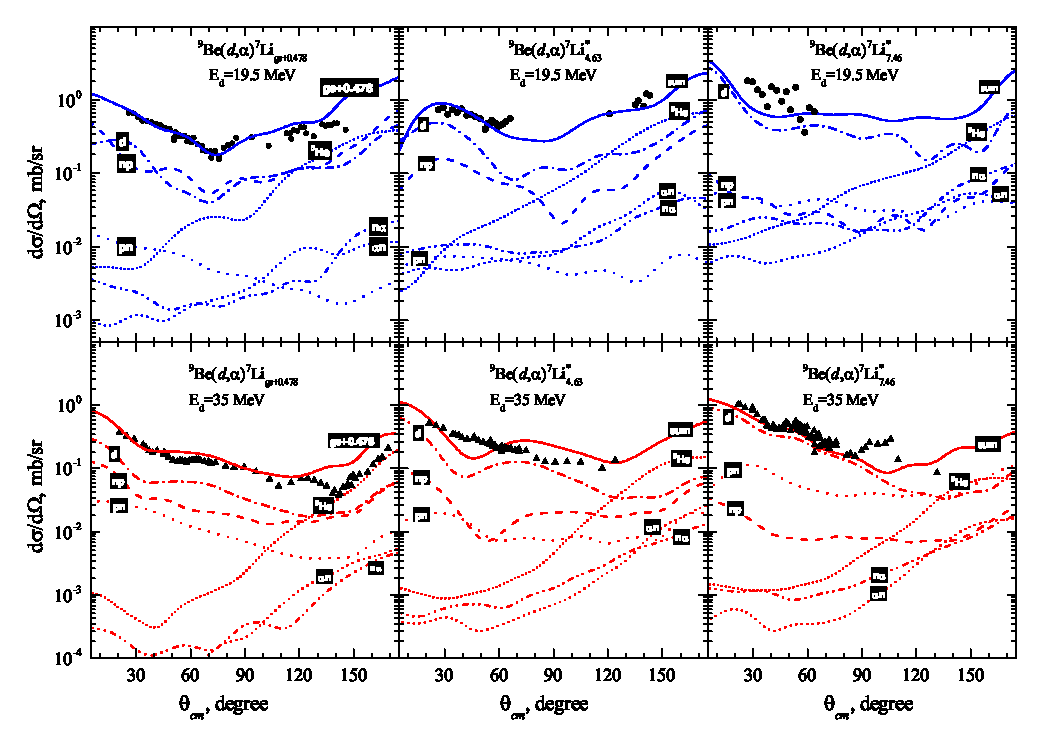
\includegraphics[scale=0.9]{4HE7LI.eps}
\caption{\label{label} Differential cross sections for the ${}^9$Be(d,$\alpha$)${}^7$Li reactions measured at 19.5 MeV and 35 MeV energy with the $^{7}$Li observed in the ground or low-lying excited states in the exit channels.}
\label{4HE7LI}
\end{figure*}	

Angular distributions of the ${}^9$Be(d,p)${}^{10}$Be nuclear reaction at E$_d$=19.5 MeV are shown in comparison with the theoretical curves in the Fig. \ref{1H10BE}.
The theoretical calculations of the direct neutron stripping carried out with the DWBA (dashed curve) underestimate the experimental data, but reproduce the behaviour well.
However, one should take into account here the couplings between d+$^9$Be and p+$^{10}$Be channels, spin re-orientations and electromagnetic transitions, which are plotted as dotted curve and marked as "CC" in Fig. \ref{1H10BE}.
Within the CRC method, i.e. taken together the latter and the DWBA calculations, we could obtain a good agreement of theoretical calculations with experimental data. It is interesting to note that we managed to describe the differential cross section of the ${}^9$Be(d,p)${}^{10}$Be$^{gs}$ nuclear reaction in all scattering angles, including the range 40$^0$-60$^0$, where they were not covered in the Ref. \cite{galanina2012, bodek1989}.

The Figure \ref{3H8BE} illustrates the cross sections of the ${}^9$Be(d,t)${}^{8}$Be nuclear reaction at both 19.5 MeV and 35 MeV energies. As in the case of the (d,p) reactions, the (d,t) reactions also show the strong channel coupling effects, especially in the ${}^9$Be(d,t)${}^{8}$Be$^{2^+}$ reaction. Theoretical calculations made within the CRC method shows good agreement with experimental data.

The results obtained within the CRC approach for the ${}^9$Be(d,p)${}^{10}$Be and ${}^9$Be(d,t)${}^{8}$Be reactions shows strong coupling effects in both entrance and exit channels. The effects of such kind were also emphasized in Ref. \cite{harakeh1980, rudchik2016}.

\begin{figure}[tp]
\centering
\includegraphics[scale=0.8]{4HE7LiCC.eps}
\caption{\label{4He7LICC} The scheme illustrates the reaction mechanisms taken into account in CRC calculations of the cross sections for ${}^9$Be(d,$\alpha$)${}^7$Li reaction.}
\end{figure}	

\subsection{Cluster transfer reaction}
Differential cross sections for the nuclear reaction ${^9}$Be(d,$\alpha$)${}^7$Li are of particular interest. The reason is in specific behaviour of the cross section at large scattering angles, that shows possibility for the ${}^5$He cluster transfer. In addition, the cross section calculated within the DWBA approach underestimates data even at forward scattering angles. Therefore, in order to cure the distinction between theory and experiment, the following transfer mechanisms are suggested (see Fig. \ref{4He7LICC}):
\begin{itemize}
\item[$-$] direct transfer of heavy clusters $d$ and ${}^5$He;
\item[$-$] sequential two-step transfer of n-p, p-n, n-$\alpha$ and $\alpha$-n;
\end{itemize}

The resulting differential cross section for the ${^9}$Be($d$,$\alpha$)${}^7$Li reaction has form of a coherent sum of two amplitudes
\begin{equation}
\frac{d\sigma}{d\Omega}(\theta) =\vert f_{I}(\theta) + f_{II}(\theta) \vert ^2,
\end{equation}
where the amplitude
\begin{equation} \label{eq:ampl1}
f_{I}(\theta)=f_{{}^5\textrm{He}}(\pi - \theta) + f_{n-\alpha}(\pi - \theta) + f_{\alpha-n}(\pi - \theta)
\end{equation}
describes the transfer of the heavy ${}^5$He-cluster and sequential two-step transfer of n-$\alpha$ and $\alpha$-n, and the amplitude
\begin{equation} \label{eq:ampl2}
f_{II}(\theta)=f_{d}(\theta) + f_{n-p}( \theta) + f_{p-n}(\theta)
\end{equation}
corresponds to the deuteron pick-up and sequential two-step transfer of n-p and p-n.

The CC potential (see Tab.~\ref{potpar}) for the entrance channel and global optical potential parameterizations from Ref. \cite{globalTriton, globalAlpha, global6Li} for intermediate and exit channels were used in the analysis.
The prior form for the first coupling, and the post form for the second coupling were chosen for two-step transfer reactions in order to avoid the non-orthogonal terms in the calculations of transition amplitudes.

%Important ingredients of the CRC method are the spectroscopic amplitudes of the composite configurations in the entrance, exit and intermediate states. In order to calculate the one nucleon spectroscopic amplitudes we applied the \textit{ANTOINE} code \cite{antoine} that reproduces the excitation functions of all p-shell nuclei well.

The spectroscopic amplitudes of the d and ${}^5$He clusters were taken from Ref. \cite{fiveSA}, while the alpha-cluster spectroscopic amplitudes given in Tab.~\ref{SA} were provided by Dr. A. Volya within the method reported in Ref. \cite{volya2017}.

The calculated cross sections are shown in Fig.~\ref{4HE7LI} with the $\alpha$-particle angular distributions formed in the ${}^9$Be(d,$\alpha$)${}^7$Li$^*$ reaction at energies 19.5 and 35 MeV and corresponding to the low-lying excitation of the ${}^7$Li nucleus in exit channels. The transfer of the deuteron (dash-dotted curve) provides the dominant contribution in all the channels. Despite the fact that the spectroscopic amplitude of the deuteron $\mathcal{S}_{1{D}_3}=0.558$ in the $^9$Be nucleus is not of great importance, a noticeable cross section is due to the large value of the deuteron spectroscopic amplitude $\mathcal{S}_{1{S}_1}=1.732$  of ${}^4$He.

The angular distribution of deuteron transfer has a significant cross section also at the back scattering angles, which is mainly caused by the contribution of the $D$ wave. This symmetrical behaviour of the cross section of $D$ waves is very similar to the cross section of evaporation residue. Tanaka et al. \cite{tanaka1978} analyzed the role of the compound process in ${}^9$Be(d,$\alpha$)${}^7$Li reaction and claimed the domination of the compond nucleus channels at the 12.17 MeV and 14.43 MeV energies. However, in Ref. \cite{bodek1989} the negligible contribution of mechanism through the compound nucleus was shown at 7 MeV using the DWBA analysis. In this regard, our theoretical results based on the CRC method shows that there is no need to take into account the mechanism through the compound nucleus at energies of 19.5 and 35.0 MeV.

In all channels starting from scattering angle $\theta_{c.m.} =$ 120$^\circ$ the transfer of the ${}^5$He cluster, labeled as ${}^5$He in Fig. \ref{4HE7LI}, has a predominant contribution. It should be noted that the similiar result was mentioned early in Ref. \cite{bodek1989}. One-step transfer of the ${}^5$He cluster was also indicated as a dominant process by Jarczyk \etal \cite{jarczyk1996} studying the ${}^{12}$C(${}^{11}$B,${}^6$Li)${}^{17}$O and ${}^{12}$C(d,${}^7$Li)${}^{7}$Be reactions.

Using the CRC method, we are able to estimate the contribution of the sequential transfer of the ${}^5$He, which was not studied before. Corresponding cross sections are shown in Fig.~\ref{4HE7LI} as curves labeled $n\alpha$ and $\alpha n$.
It turned out that the $n\alpha$ and the $\alpha n$ transfer processes provide indeed the contribution more than one order of magnitude lower in comparison with the one-step ${}^5$He transfer. Nevertheless, it should be noted that the contribution of the n-$\alpha$ and the $\alpha$-n transfer channels increases with the ${}^7$Li excitation increases, where they should not be ignored.

\begin{figure}%[tp]
\centering
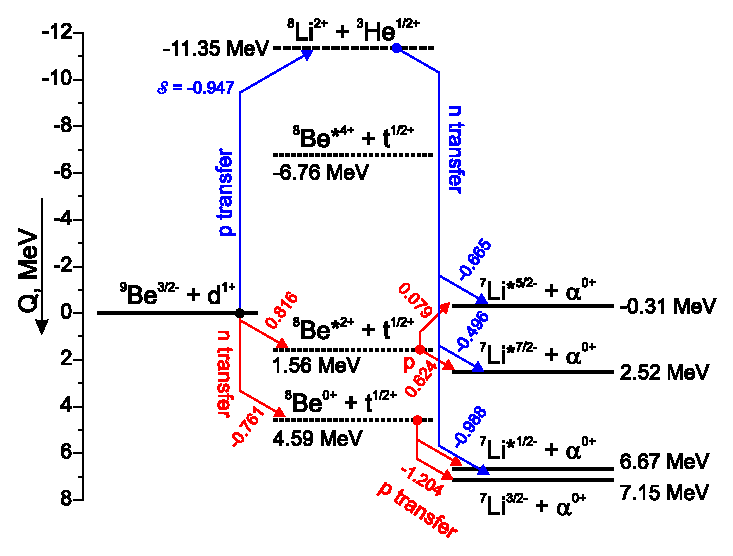
\includegraphics[width=230pt]{pnvsnp.eps}
\caption{\label{fig:pnvsnp} The scheme illustrates the energy balance of the different intermediate stages for the two-step mechanisms of ${}^9$Be(d,$\alpha$)${}^7$Li transfer reaction. The $Q$-values for the different intermediate channels are shown near the corresponding lines. The numbers near the arrows correspond to the spectroscopic amplitudes of the heaviest reaction participants. For example, spectroscopic amplitude for the ${}^9$Be = ${}^8$Li + p configuration is equal $\mathcal{S} = -0.947$.}
\end{figure}

The two-step n-p transfer is another mechanism providing noticeable contribution to the cross section. It is due to the prominent cluster structure of the ${}^9$Be nucleus having the weakly bound neutron. This structural feature explains also the weakness of the p-n sequential transfer contribution to the cross section corresponding the ${}^7$Li(g.s.) in the exit channel. However curves in Fig.~\ref{fig:pnvsnp} with increasing the ${}^7$Li excitation energy these two mechanisms change their places and the p-n transfer begins to play a leading role, providing, in particular, almost 10 times large contribution in the case of reaction at the $E_{lab}$ = 35 MeV with ${}^7$Li$^*$(7.46 MeV) in exit channel.

In Fig.~\ref{fig:pnvsnp} the possible scenarios of the n-p and p-n sequential transferring for the reaction under consideration are shown in respect to the $Q$-values. One may see that all the steps of the n-p sequential transfer have the positive $Q$-values, while the p-n transfer goes through the intermediate channel ${}^8$Li + ${}^3$He having considerable negative $Q$-value. Together with large values of the spectroscopic amplitudes (shown near the arrows in Fig. \ref{fig:pnvsnp}) it explains the leading role of the (d,t;t,$\alpha$) mechanism in populating the ground state of the ${}^7$Li in the exit channel.

The situation becomes quite different in the case of the ${}^7$Li$^*$(5/2$^-$) in the exit channel. First of all the population of this state through the n-p transferring includes the ${}^9$Be~=~${}^8$Be$^*(2^+)$~+~n intermediate configuration where ${}^8$Be cluster has to be in $2^+$ excited state. Note that the ${}^8$Be($0^+$) ground state is inappropriate because of angular momentum coupling mismatch in entrance and exit configurations. Second circumstance is an extremely small spectroscopic amplitude of the ${}^8$Be$^*(2^+)$~=~${}^7$Li$^*(5/2^-)$~+~p configuration which is equal $\mathcal{S} = 0.079$. These two factors lead to the suppression of the contribution of (d,t;t,$\alpha$) mechanism in population of the ${}^7$Li$^*$(5/2$^-$) state in the exit channel. Therefore the p-n sequential transfer prevails over the n-p one. With rising the collision energy the suppression of the (d,t;t,$\alpha$) mechanism is even enhanced due to decrease the reaction time while the presence of the ${}^8$Be$^*(2^+)$ intermediate state indicates that the process actually becomes multi-step one that requires more time.

Figure \ref{CS} shows the results of calculations of the integrated cross sections for each mechanism in the ${}^9$Be(d,$\alpha$)${}^7$Li$^{gs}$ nuclear reaction. The contribution to the cross section can be made in the following order: direct transfer of the deuteron, transfer of the n-p system, transfer of a heavy ${}^5$He cluster,  and sequential transfer of the p-n, a-n, and n-a systems. However, the order of the contribution of the p-n and ${}^5$He mechanisms changes when the laboratory energy reaches a value of 100 MeV. If one does not take into account the correlations of the $\alpha+^7$Li output channel, the high value of the spectroscopic amplitude of the deuteron in the $\alpha$ particle, then we can conclude that the ground state of the $^9$Be nucleus has a cluster configuration $n+^8$Be, and then $\alpha+^5$He. Such kind of conclution agrees well with the experimental studies \cite{brown2007, papka2007}.
%The results of calculations show that the more excitation energy of the ${}^7$Li nucleus, the less contribution of the n-p system is given, the more contribution of the p-n system.

\begin{figure}[tp]
\centering
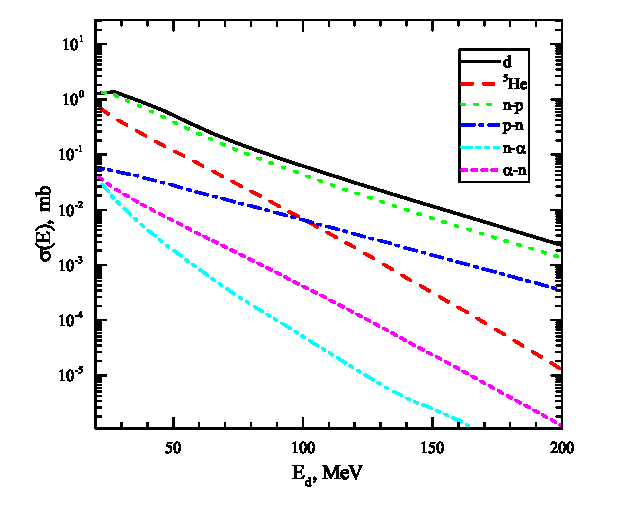
\includegraphics[width=8.2cm]{CS.eps}
\caption{\label{CS} Integrated cross sections depending on laboratory energy E$_d$ for each mechanism: d, ${}^5$He, n-p, p-n, n-$\alpha$ and $\alpha$-n. }
\end{figure}	
	
\section{Conclusion}
In the present work, the nuclear reactions induced by interaction of deuteron with ${}^9$Be  have been analysed. The following conclusions can be made during the analysis:
\begin{itemize}
\item The double-folding potential, which is characteristic of the interaction of deuteron with ${}^9$Be, differs from phenomenological optical potentials;
\item  The deformation parameter has been obtained for the excited state 2.43 MeV of ${}^9$Be;
\item The strong coupling effects in the nuclear reactions with one nucleon transfer have been revealed;
\item It was found that  in the ${}^9$Be(d,$\alpha$)${}^7$Li nuclear reaction the ${}^5$He heavy cluster  is transferred mainly simultaneously, and the contribution of its sequential transfer is an order of magnitude lower;
\item The importance of taking into account the mechanism of sequential transfer of the n-p system has been revealed.
\end{itemize}

\ack
	The authors acknowledge the support of the CANAM project \cite{canam} for providing beam time for the experiment. The authors also grateful to I. Thompson for advising on FRESCO code and to A. Volya for giving the alpha spectroscopic amplitudes.

This work was supported by the Russian Science Foundation (17-12-01170).
%and by the Program of the Ministry of Education and Science of Kazakhstan (IRN~AP05132978)



\section*{References}

\bibliographystyle{iopart-num}
%\begin{thebibliography}
\bibliography{urazbekov}
%\end{thebibliography}

\end{document}